\documentclass{sigchi}

\newcommand{\inlinequote}[1]{\textit{``#1''}}

% Use this command to override the default ACM copyright statement
% (e.g. for preprints).  Consult the conference website for the
% camera-ready copyright statement.

%% HOW TO OVERRIDE THE DEFAULT COPYRIGHT STRIP --
%% Please note you need to make sure the copy for your specific
%% license is used here!
 \toappear{
 Team De Fr\'{e}Fr\'{e}~\copyright{}~2016
 %Permission to make digital or hard copies of all or part of this work for personal or classroom use is granted without fee provided that copies are not made or distributed for profit or commercial advantage and that copies bear this notice and the full citation on the first page. Copyrights for components of this work owned by others than ACM  must be honored. Abstracting with credit is permitted. To copy otherwise, or republish, to post on servers or to redistribute to lists, requires prior specific permission and/or a fee. Request permissions from \href{mailto:Permissions@acm.org}{Permissions@acm.org}. \\
 %\emph{CHI '16},  May 07--12, 2016, San Jose, CA, USA \\
 %ACM xxx-x-xxxx-xxxx-x/xx/xx\ldots \$15.00 \\
 %DOI: \url{http://dx.doi.org/xx.xxxx/xxxxxxx.xxxxxxx}
}

% Arabic page numbers for submission.  Remove this line to eliminate
% page numbers for the camera ready copy
% \pagenumbering{arabic}

% Load basic packages
\usepackage{balance}       % to better equalize the last page
\usepackage{graphics}      % for EPS, load graphicx instead 
\usepackage[T1]{fontenc}   % for umlauts and other diaeresis
\usepackage{txfonts}
\usepackage{mathptmx}
\usepackage[pdflang={en-US},pdftex]{hyperref}
\usepackage{color}
\usepackage{booktabs}
\usepackage{textcomp}
\usepackage{pdfpages}


% Some optional stuff you might like/need.
\usepackage{microtype}        % Improved Tracking and Kerning
% \usepackage[all]{hypcap}    % Fixes bug in hyperref caption linking
\usepackage{ccicons}          % Cite your images correctly!
% \usepackage[utf8]{inputenc} % for a UTF8 editor only

% If you want to use todo notes, marginpars etc. during creation of
% your draft document, you have to enable the "chi_draft" option for
% the document class. To do this, change the very first line to:
% "\documentclass[chi_draft]{sigchi}". You can then place todo notes
% by using the "\todo{...}"  command. Make sure to disable the draft
% option again before submitting your final document.
\usepackage{todonotes}

% Paper metadata (use plain text, for PDF inclusion and later
% re-using, if desired).  Use \emtpyauthor when submitting for review
% so you remain anonymous.
\def\plaintitle{Salon de Fr\'{e}Fr\'{e}: A VR + ASMR Experience}
\def\plainauthor{Ryan Bluth, Michael Hetman, Sean LeBlanc,
  Kiera Lundberg, Emma Thurlow, Catherine Wong}
\def\emptyauthor{}
\def\plainkeywords{Virtual Reality; VR; Virtual Environments; Autonomous Sensory Meridian Response; ASMR; Presence; Immersion; Head-Mounted Display; HMD; Flow State; Treatment; Therapy}{}
\def\plaingeneralterms{Documentation, Standardization}

% llt: Define a global style for URLs, rather that the default one
\makeatletter
\def\url@leostyle{%
  \@ifundefined{selectfont}{
    \def\UrlFont{\sf}
  }{
    \def\UrlFont{\small\bf\ttfamily}
  }}
\makeatother
\urlstyle{leo}

% To make various LaTeX processors do the right thing with page size.
\def\pprw{8.5in}
\def\pprh{11in}
\special{papersize=\pprw,\pprh}
\setlength{\paperwidth}{\pprw}
\setlength{\paperheight}{\pprh}
\setlength{\pdfpagewidth}{\pprw}
\setlength{\pdfpageheight}{\pprh}

% Make sure hyperref comes last of your loaded packages, to give it a
% fighting chance of not being over-written, since its job is to
% redefine many LaTeX commands.
\definecolor{linkColor}{RGB}{6,125,233}
\hypersetup{%
  pdftitle={\plaintitle},
% Use \plainauthor for final version.
%  pdfauthor={\plainauthor},
  pdfauthor={\emptyauthor},
  pdfkeywords={\plainkeywords},
  pdfdisplaydoctitle=true, % For Accessibility
  bookmarksnumbered,
  pdfstartview={FitH},
  colorlinks,
  citecolor=black,
  filecolor=black,
  linkcolor=black,
  urlcolor=linkColor,
  breaklinks=true,
  hypertexnames=false
}

% create a shortcut to typeset table headings
% \newcommand\tabhead[1]{\small\textbf{#1}}

% End of preamble. Here it comes the document.
\begin{document}

\title{\plaintitle}

\numberofauthors{3}
\author{%
  \alignauthor{Ryan Bluth\\
    \email{ryan.bluth@carleton.ca}}\\
  \alignauthor{Michael Hetman\\
    \email{michael.hetman@carleton.ca}}\\
  \alignauthor{Sean LeBlanc\\
    \email{sean.leblanc@carleton.ca}}\\
  \alignauthor{Kiera Lundberg\\
    \email{kiera.lundberg@carleton.ca}}\\
  \alignauthor{Emma Thurlow\\
    \email{emma.thurlow@carleton.ca}}\\
  \alignauthor{Cartherine Wong\\
    \email{catherine.wong@carleton.ca}}\\
}

\maketitle

\begin{abstract}
We will build a multimedia experience which combines VR with ASMR and plan to compare users' experiences with the VR system against an audio-only system. We expect to see higher levels of relaxation as a result of the increased immersion/presence offered by VR.
\end{abstract}

\keywords{\plainkeywords}

\category{H.5.1}{Multimedia Information Systems: Artificial, augmented, and virtual realities}{}{}

\section{Introduction}

\subsection{Project Overview}

The topic of interest for this project is Autonomous Sensory Meridian Response, commonly known as ASMR, which is a \inlinequote{sensory phenomenon, in which individuals experience a tingling, static-like sensation across the scalp, back of the neck and at times further areas in response to specific triggering audio and visual stimuli}~\cite{barratt2015autonomous}. Although ASMR can occur as a result of virtually any stimulus, there is an emerging trend of ASMR content uploaded to YouTube, with one of the most popular channels garnering nearly 200 million views since their first video was uploaded four years ago~\cite{anon.gentlewhispering}. These videos are meant to lull viewers into relaxed states by incorporating specific audio stimuli, including whispering, tapping, brushing, and other sounds, ideally recorded using binaural microphones for increased immersion.

\begin{figure}[htb]
\centering
  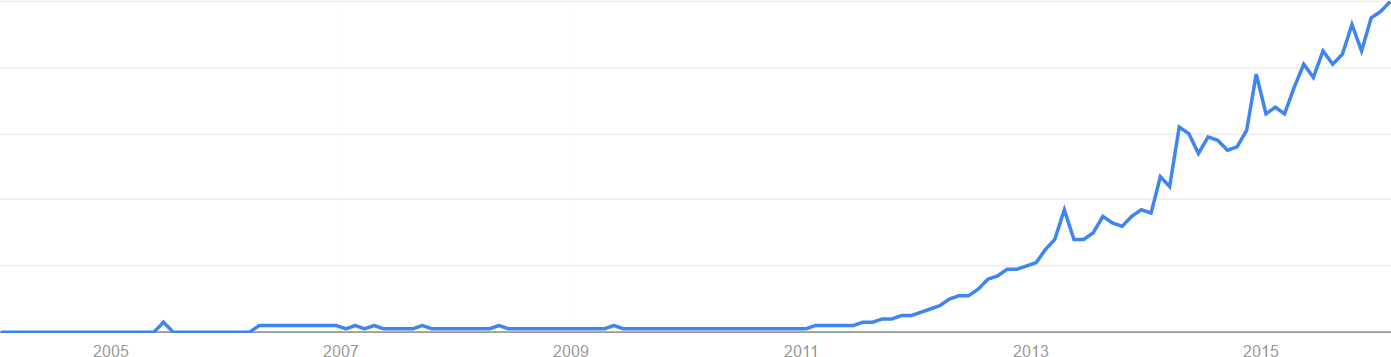
\includegraphics[width=0.9\columnwidth]{figures/google-trends}
  \caption{The popularity of ASMR searches has been rising steadily over the past four years. Data Source: Google Trends (\url{www.google.com/trends/}).}~\label{fig:google-trends}
\end{figure}

We plan to explore whether the immersion, presence, and/or interactivity of a virtual reality system affects viewers' experience with media designed to evoke ASMR. This exploration will be achieved through the use of a custom-developed ASMR experience, an Oculus Rift\footnote{DK2 headset}, and a pair of high quality headphones\footnote{Grado SR80e headphones}.

The ASMR experience that we intend to create is one wherein the participant's avatar receives a virtual salon makeover. It will consist of a makeup artist, shown in proxy as a roughly animated character silhouette, applying makeup to the participant's avatar. True to the format of ASMR videos, the artist will move around and speak as they go about their tasks. The artist's speech will be a pre-recorded mono track and positional audio will be used to place it relative to the participant.

\begin{figure}[htb]
\centering
  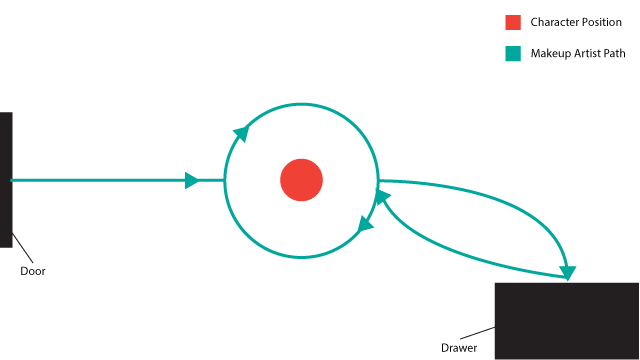
\includegraphics[width=0.9\columnwidth]{figures/layout}
  \caption{Mockup of the salon layout and the makeup artist's motion path.}~\label{fig:layout}
\end{figure}

At certain points, the artist will offer participants a selection of products. A selection can be made by through head-tracking: by maintaining eye contact with the choice for a set time (see
Figure~\ref{fig:selection}). Choices made will cosmetically affect the avatar displayed at the experience's conclusion.

\begin{figure}[htb]
\centering
  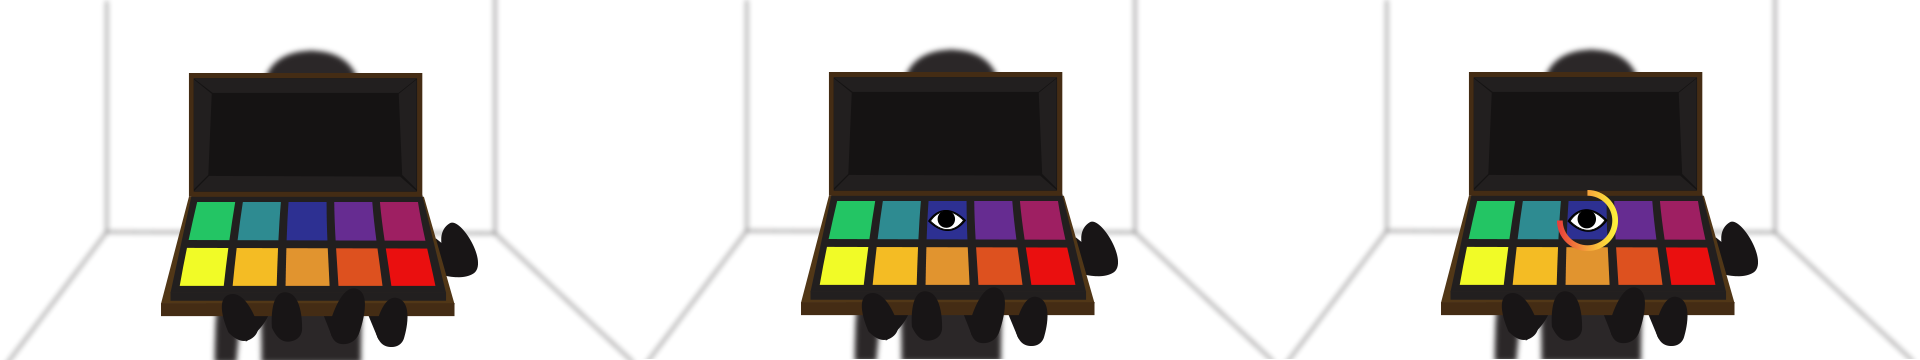
\includegraphics[width=0.9\columnwidth]{figures/selection}
  \caption{Mockup of the selection method which uses the center of the screen as a cursor position.}~\label{fig:selection}
\end{figure}

\subsection{User Study}

To evaluate the experience, a comparative study will be performed in which participants are exposed to two variations of the experience: one will be the VR experience exactly as developed, and the other will lack visual stimuli and interaction in order to isolate audio, the component most closely associated with the YouTube ASMR format\footnote{During interactive elements in which a question is posed to the participant, the audio will continue without any user input. Both versions will include some questions in this format (e.g. \inlinequote{How was your day?}) to avoid interference with study results.}. The test will use a within-subjects design, as individual differences would be a significant source of error for something as subjective as ASMR.

We hypothesize that the addition of visual stimuli and interaction with the system will further immerse the participant in the ASMR experience. As 98\% of individuals searching for ASMR videos have indicated that they do so for relaxation~\cite{barratt2015autonomous}, we will be evaluating the participant's sense of relaxation. This will be measured through surveys and possible physiological indicators (e.g. heart rate, respiratory rate) during or after the experience. We expect to observe higher satisfaction with the experience as a result of these factors than with passive audio alone. We believe this will open up the ASMR video-producing community to a new form of experience unlike those found on YouTube.

\subsection{Future Work}

A possible extension of this experience would be to have the test administrator brush the participant's face with actual makeup brushes in-sync with the virtual brushes. As we intend to primarily evaluate the visual and interactive elements, this idea was excluded from this proposal. We hypothesize that this haptic stimuli on its own could be capable of eliciting sensations similar to ASMR (which would interfere with our study)~\cite{hall1897psychology}, and so we leave this for future works to consider.

\subsection{Experience Outline}

\begin{enumerate}
\item{The participant is seated and puts on the equipment}
\item{A makeup artist enters the salon and introduces herself}
\item{The artist asks participants to select a colour for their makeup}
\begin{itemize}
\item{VR: Participants are presented with a palette and make a selection}
\end{itemize}
\item{The artist circles participants, brushing their face and whispering quietly about what she's doing, occasionally complimenting the participant}
\item{Participants are informed that the makeup is complete }
\item{The artist instructs participants to turn and look at their reflection in a mirror she's holding}
\begin{itemize}
\item{VR: Participants see their avatar in a mirror, re-textured based on earlier selections}
\end{itemize}
\end{enumerate}

\section{Related Work}

\subsection{Introduction to Autonomous Sensory Meridian Response}
Autonomous Sensory Meridian Response (ASMR, is the tingling sensation across the scalp and back of the neck, caused by specific audio and visual stimuli~\cite{barratt2015autonomous}. To experience ASMR, many users watch videos, often involving personal attention or grooming role-play \cite{andersen2015now,barratt2015autonomous} with a female host~\cite{andersen2015now} designed to elicit the phenomenon. Various types of stimuli can be used within a video to evoke the desired response~\cite{barratt2015autonomous}. When surveying those that experienced ASMR in order to learn which stimuli was triggering, it was found that whispering, personal attention, crisp sounds, and slow movements could cause the response. Whispering was the most common among participants, affecting 75\% \cite{barratt2015autonomous}. To increase the sensation, users may change their environment by dimming the lights or using headphones~\cite{begman2015}. For our project, we will be recording similar audio stimuli to those listed above, and utilizing high-fidelity headphones for the best experience. Since an HMD will be used, dimming the lights is unnecessary.

Apart from eliciting a tingling sensation, ASMR is able to put users into a state similar to flow state, \inlinequote{the state of intense focus and diminished awareness of the passage of time that is often associated with optimal performance}~\cite{barratt2015autonomous}. During their research, Barratt and Davis observed that this state of concentration was improved with more ASMR triggers~\cite{barratt2015autonomous}. ASMR is valued for its calming effects \cite{barratt2015autonomous}; polls indicated that 98\% of users view ASMR videos for relaxation, and 70\% for stress relief~\cite{barratt2015autonomous}. Some believe in its effects enough to promote ASMR as a treatment for stress-related conditions such as anxiety~\cite{andersen2015now,begman2015}.

Unfortunately for those who use ASMR, these effects can be lost over long-time usage~\cite{andersen2015now}. In this situation, users often turn to more immersive experiences that use binaural sound and 3D microphones~\cite{andersen2015now}. It is believed that this adds to the experience's intimacy, heightening the response~\cite{andersen2015now}. We hope to determine whether the increased level of immersion of our choice of display will amplify the sensations provided by ASMR.

\subsection{Virtual Reality Input Methods}
In a 2008 study, when comparing mouse and gaze pointing methods, participants perceived gaze as faster but less accurate than mouse pointing~\cite{mateo2008gaze}. Discomfort is a drawback of gaze pointing, especially if users must keep their heads still for a long time~\cite{mateo2008gaze}. We believe that the gaze method will work well for our project, as users will not be asked to complete tasks requiring accuracy or holding a position for a long time.

\subsection{The Effects of Virtual Reality}
Like real life environments, virtual environments can cause emotional reactions. During a 2007 experiment, it was found that when placed into a relaxation- or anxiety-inducing environment, participants showed signs of either relaxation or anxiety~\cite{riva2007affective}. It was also shown that a relaxing VR experience can increase feelings of quietness and happiness while reducing anger, sadness and anxiety~\cite{riva2007affective}. This suggests that virtual environments can be designed to evoke an emotional response from users~\cite{riva2007affective,wiederhold2006evaluation}. 
It was also found that the level of presence\footnote{\inlinequote{the \inlinequote{sense of being there} or the \inlinequote{feeling of being in a world that exists outside the self.}}~\cite{riva2007affective}} felt by participants was greater in relaxing and anxious environments than in neutral ones, and that the greatest feeling of presence was achieved in the relaxing environment~\cite{riva2007affective}. A previous review of virtual environments found that a participant's sense of presence is influenced by the attributes of the VR platform, the features of the environment itself, and the individuals characteristics~\cite{nash2000review}.

VR has also been seen as an alternative to therapy administration, which could help people in overcoming anxiety and stress-related conditions. It has been found in various studies that individuals enjoy VR therapy more than traditional therapy, leading to an increase in motivation to complete treatment~\cite{kizony2003adapting,morel2015advantages}. VR therapy also has the benefit of current equipment being affordable, allowing participants to engage in sessions in their own homes~\cite{morel2015advantages}. When researching the viability of VR therapy, a follow-up survey of those who suffered from anxiety found that there was no significant difference in the level of anxiety felt between participants of VR and traditional therapy~\cite{safir2011virtual}.

VR and ASMR have the shared capability of inducing relaxation and are both often used for therapeutic purposes. We hope that by combining these two relaxing mediums, users will be able to achieve a higher level of presence, which will increase the perception of intimacy ASMR users desire, leading to an increase in its effects.

\subsection{Testing Methods}
To collect data on subjective topics, questionnaires are a useful tool. During Riva's experiment on the link between presence and emotions in multiple virtual environments, questionnaires were used to evaluate mood before and after the experience including Visual Analogue Scale (VAS), Positive and Negative Affect Schedule (PANAS), and State Trait Anxiety Inventory (STAI). The VAS required participants to indicate how they feel at a specific moment in time regarding their level of happiness, anger, surprise, disgust, anxiety and quietness. The PANAS uses a list of 20 adjectives that describe 10 positive and 10 negative emotions which can be viewed in Appendix~\ref{Appendix_A}. Participants must associate a magnitude on a scale of 1-5 for each emotion at a given moment. The STAI measures the level of anxiety participants feel on a scale of 0-3. The \inlinequote{State} version of this questionnaire asks participants how they feel at a given moment, while the \inlinequote{Trait} version asks for their general feelings. These questionnaires were provided to participants before and after testing to compare their baseline emotional state against the effects of the environment. Two additional questionnaires, the UCL Presence Questionnaire, and the Independent Television Company Sense of Presence Inventory (ITC-SOPI) were also given to participants after each stage in order to assess their presence. For the UCL Presence Questionnaire, please see Appendix~\ref{Appendix_A}.
The ITC-SOPI was used to measure different dimensions of presence, such as sense of physical space, engagement, ecological validity, and negative effects. The questionnaire is divided into two parts. The first consists of six items used to measure a participant's experience after the test has concluded, and the second consists of 38 items used to measure the participants experience during the test. Each is scored using a 5-point Likert scale~\cite{riva2007affective}.

Riva and her team also asked participants questions rated using a 10-point scale, while they were within the virtual environment. To measure their emotional status, participants were asked to what extent they felt sad, happy, anxious, and relaxed at any given moment. To measure presence, participants were asked if they felt as if they were in the virtual environment and whether that environment was a real place they were visiting. To view these questions, please see Appendix~\ref{Appendix_A}.
To reduce errors as a result of their within-subjects design, every participant was required to test each environment, with the sequence of environments being randomized~\cite{riva2007affective}.

For objective measurements on the emotional state of participants, physiological measures, such as heart-rate, can be taken. During a 2006 study on the effects of relaxation techniques and heart rate variability, it was found that guided relaxation decreased the participant's heart rate~\cite{sarang2006effects}. This shows a correlation between an individual's level of relaxation, which cannot directly be measured, and their heart rate.

To gather information on \inlinequote{the prevalence of particular features of ASMR, when and why individuals engage in ASMR, and the relation of ASMR to other known phenomenon}, Barratt and Davis collected information on a participant's viewing habits and various facets of their experience using a questionnaire~\cite{barratt2015autonomous}. Although this questionnaire is designed for use with those already familiar with ASMR, it could likely be used to assess the experiences of individuals new to the phenomenon. A version of the original questionnaire can be found in Appendix~\ref{Appendix_A}. 



\section{Methodology}

\subsection{Participants}
The experiment was completed by 10 participants. The average age was 21.67 years old with a standard deviation of 1.41. Of the 10 participants, 6 were male, 3 were female, and 1 identifies as another gender. All of the participants except for 1 had previous experience using VR. Three participants had previously experienced ASMR, listing their triggers as whispering and personal attention, whispering and crisp sounds, and crisp sounds respectively. None of the participants indicated that they watch ASMR videos in their daily life.

Of the 10 participants, one was excluded from the study as they indicated they had a history of heart problems in the family and suffered from a heart condition.

\subsection{Apparatus}
\begin{itemize}
\item{Oculus Rift DK2 (note: only the HMD's tracking is used; the external tracker which provides positional data is ignored for the purposes of this study)}
\item{S-Tengine2 game engine + "Salon de Fr\'{e}Fr\'{e}" application
\begin{itemize}
\item{60 FPS}
\item{~30 ms latency}
\end{itemize}
}
\item{Grado SR80e headphones}
\item{Garmin FORERUNNER 410 + heart rate monitor attachment}
\item{Laptop
\begin{itemize}
\item{Windows 10 64-bit}
\item{16 GB RAM}
\item{Intel Core i7-3610QM CPU @ 2.30GHz 2.30 GHz}
\item{NVIDIA GeForce GTX 670M}
\end{itemize}
}
\end{itemize}

\subsection{Procedure}
Participants were read a script, included in the Appendix, that informed them about the ASMR phenomenon, as well as the procedure they would have to follow during the test. They completed a pre-screening questionnaire to provide background information that may affect the test, and were asked to sign a consent form.

Participants were then asked to complete the two procedures outlined below. The order of these tests was alternated between participants to account for any confounding variables caused by completing tests in the same order.

The experiment took an average of 20 minutes to complete per participant.

\subsubsection{Virtual Reality + Audio}
\begin{enumerate}
\item{The participant is seated and puts on the HMD and headphones}
\item{A makeup artist introduces herself}
\item{The artist asks participants to select a blush colour}
\item{Participants are presented with a palette and make a selection by looking at the option they want}
\item{The artist asks participants to select an eyeshadow colour}
\item{Participants are presented with a palette and make a selection by looking at the option they want}
\item{The artist asks participants to select an eyeliner colour}
\item{Participants are presented with a palette and make a selection by looking at the option they want}
\item{The artist asks participants to select a lipstick colour}
\item{Participants are presented with a palette and make a selection by looking at the option they want}
\item{Participants are informed that the makeup is complete and are told to look in the mirror}
\item{Participants remove HMD}
\item{Participants complete a questionnaire}
\end{enumerate}

\subsubsection{Audio-only}
\begin{enumerate}
\item{The participant is seated and puts on the HMD and headphones}
\item{An audio file containing the entire experience is played}
\item{Participants remove HMD}
\item{Participants complete a questionnaire}
\end{enumerate}

\section{}

%\section{Sample stuff}

%\begin{table}[htb]
  %\centering
 % \begin{tabular}{l r r r}
    % \toprule
 %   & & \multicolumn{2}{c}{\small{\textbf{Test Conditions}}} \\
 %   \cmidrule(r){3-4}
 %   {\small\textit{Name}}
 %   & {\small \textit{First}}
%      & {\small \textit{Second}}
 %   & {\small \textit{Final}} \\
  %  \midrule
  %  Marsden & 223.0 & 44 & 432,321 \\
  %  Nass & 22.2 & 16 & 234,333 \\
  %  Borriello & 22.9 & 11 & 93,123 \\
  %  Karat & 34.9 & 2200 & 103,322 \\
    % \bottomrule
%  \end{tabular}
%  \caption{Table captions should be placed below the table. We
%    recommend table lines be 1 point, 25\% black. Minimize use of
%    table grid lines.}~\label{tab:table1}
%\end{table}


%\begin{figure*}[htb]
%  \centering
%  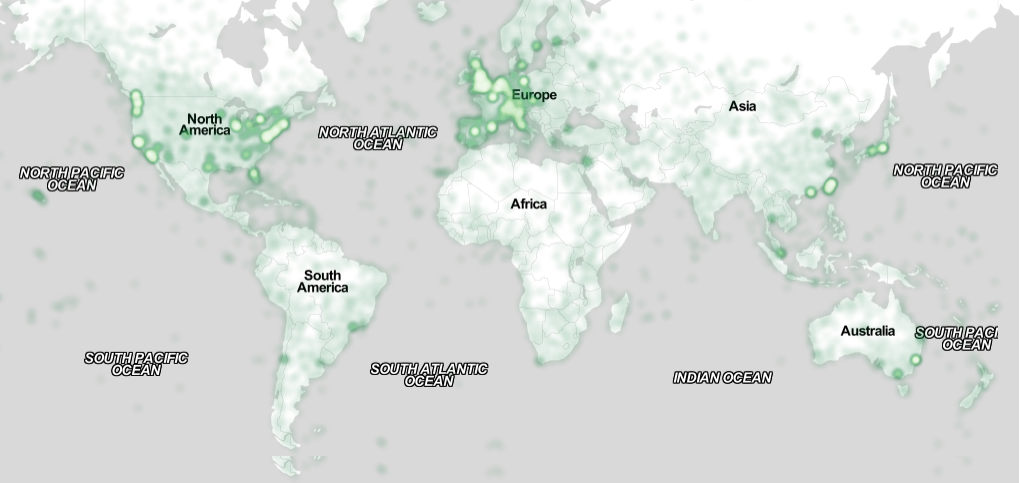
\includegraphics[width=1.75\columnwidth]{figures/map}
%  \caption{In this image, the map maximizes use of space. You can make
%    figures as wide as you need, up to a maximum of the full width of
%    both columns. Note that \LaTeX\ tends to render large figures on a
%    dedicated page. Image: \ccbynd~ayman on
%    Flickr.}~\label{fig:figure2}
%\end{figure*}

% Balancing columns in a ref list is a bit of a pain because you
% either use a hack like flushend or balance, or manually insert
% a column break.  http://www.tex.ac.uk/cgi-bin/texfaq2html?label=balance
% multicols doesn't work because we're already in two-column mode,
% and flushend isn't awesome, so I choose balance.  See this
% for more info: http://cs.brown.edu/system/software/latex/doc/balance.pdf
%
% Note that in a perfect world balance wants to be in the first
% column of the last page.
%
% If balance doesn't work for you, you can remove that and
% hard-code a column break into the bbl file right before you
% submit:
%
% http://stackoverflow.com/questions/2149854/how-to-manually-equalize-columns-
% in-an-ieee-paper-if-using-bibtex
%
% Or, just remove \balance and give up on balancing the last page.
%
\balance{}

% BALANCE COLUMNS
\balance{}

% REFERENCES FORMAT
% References must be the same font size as other body text.
\bibliographystyle{SIGCHI-Reference-Format}
\bibliography{sample}

\appendix
\section{Appendix A - Test Materials}\label{Appendix_A}
\subsection{UCL Presence Questionnaire}
For the UCL Presence Questionnaire, subjects were asked to answer using a 1-7 point Likert scale for the following questions:
\begin{enumerate}
	\item{\inlinequote{Rate your sense of being in the virtual environment.}}
	\item{\inlinequote{To what extent were there times during the experience when the virtual environment was reality for you?.}}
	\item{\inlinequote{When you think back to the experience, do you think of the virtual environment more as images that you saw or more	as somewhere that you visited?}}
	\end{enumerate}

\subsection{Affective Interactions Using Virtual Reality - Emotional Status and Presence Questionnaire}
To measure their emotional status, the following questions were asked:
\begin{enumerate}
	\item{\inlinequote{To what extent do you feel sad at this moment?}}
	\item{\inlinequote{To what extent do you feel happy at this	moment?}}
	\item{\inlinequote{To what extent do you feel anxious at this moment?}}
	\item{\inlinequote{To what extent do you feel relaxed at this moment?}}
\end{enumerate}

To measure presence, the following questions were asked:
\begin{enumerate}
	\item{\inlinequote{Do you feel you are here, in [the environment portrayed with virtual reality]?}}
	\item{\inlinequote{Do you feel this [virtual environment] is real, is it a place you are visiting?}}
\end{enumerate}

\subsection{Positive and Negative Affect Schedule}
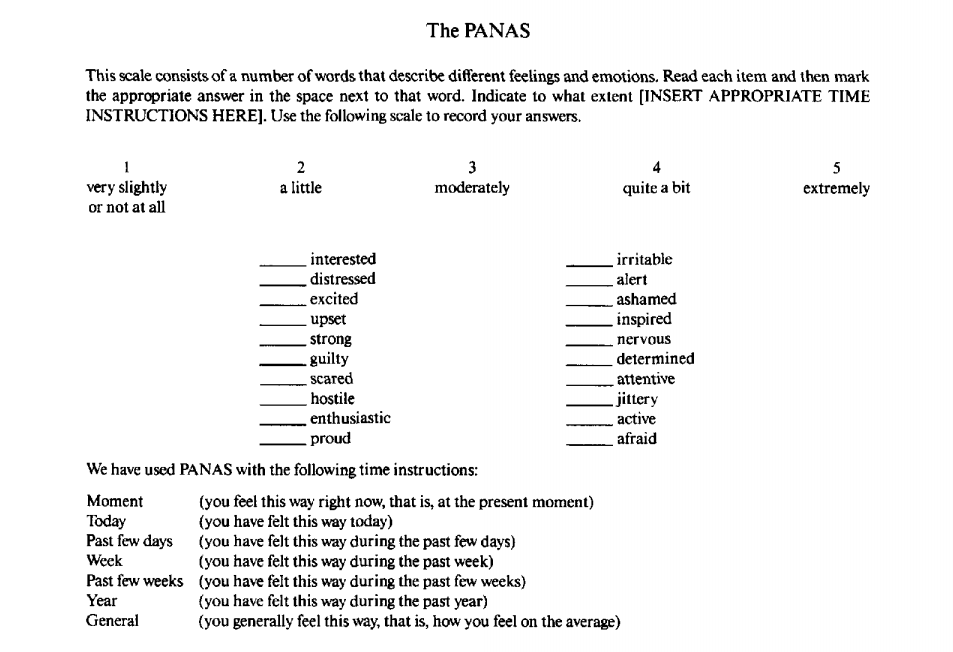
\includegraphics[width=0.5\textwidth]{questionnaires/ThePANAS.png}

\subsection{ASMR Questionnaire}
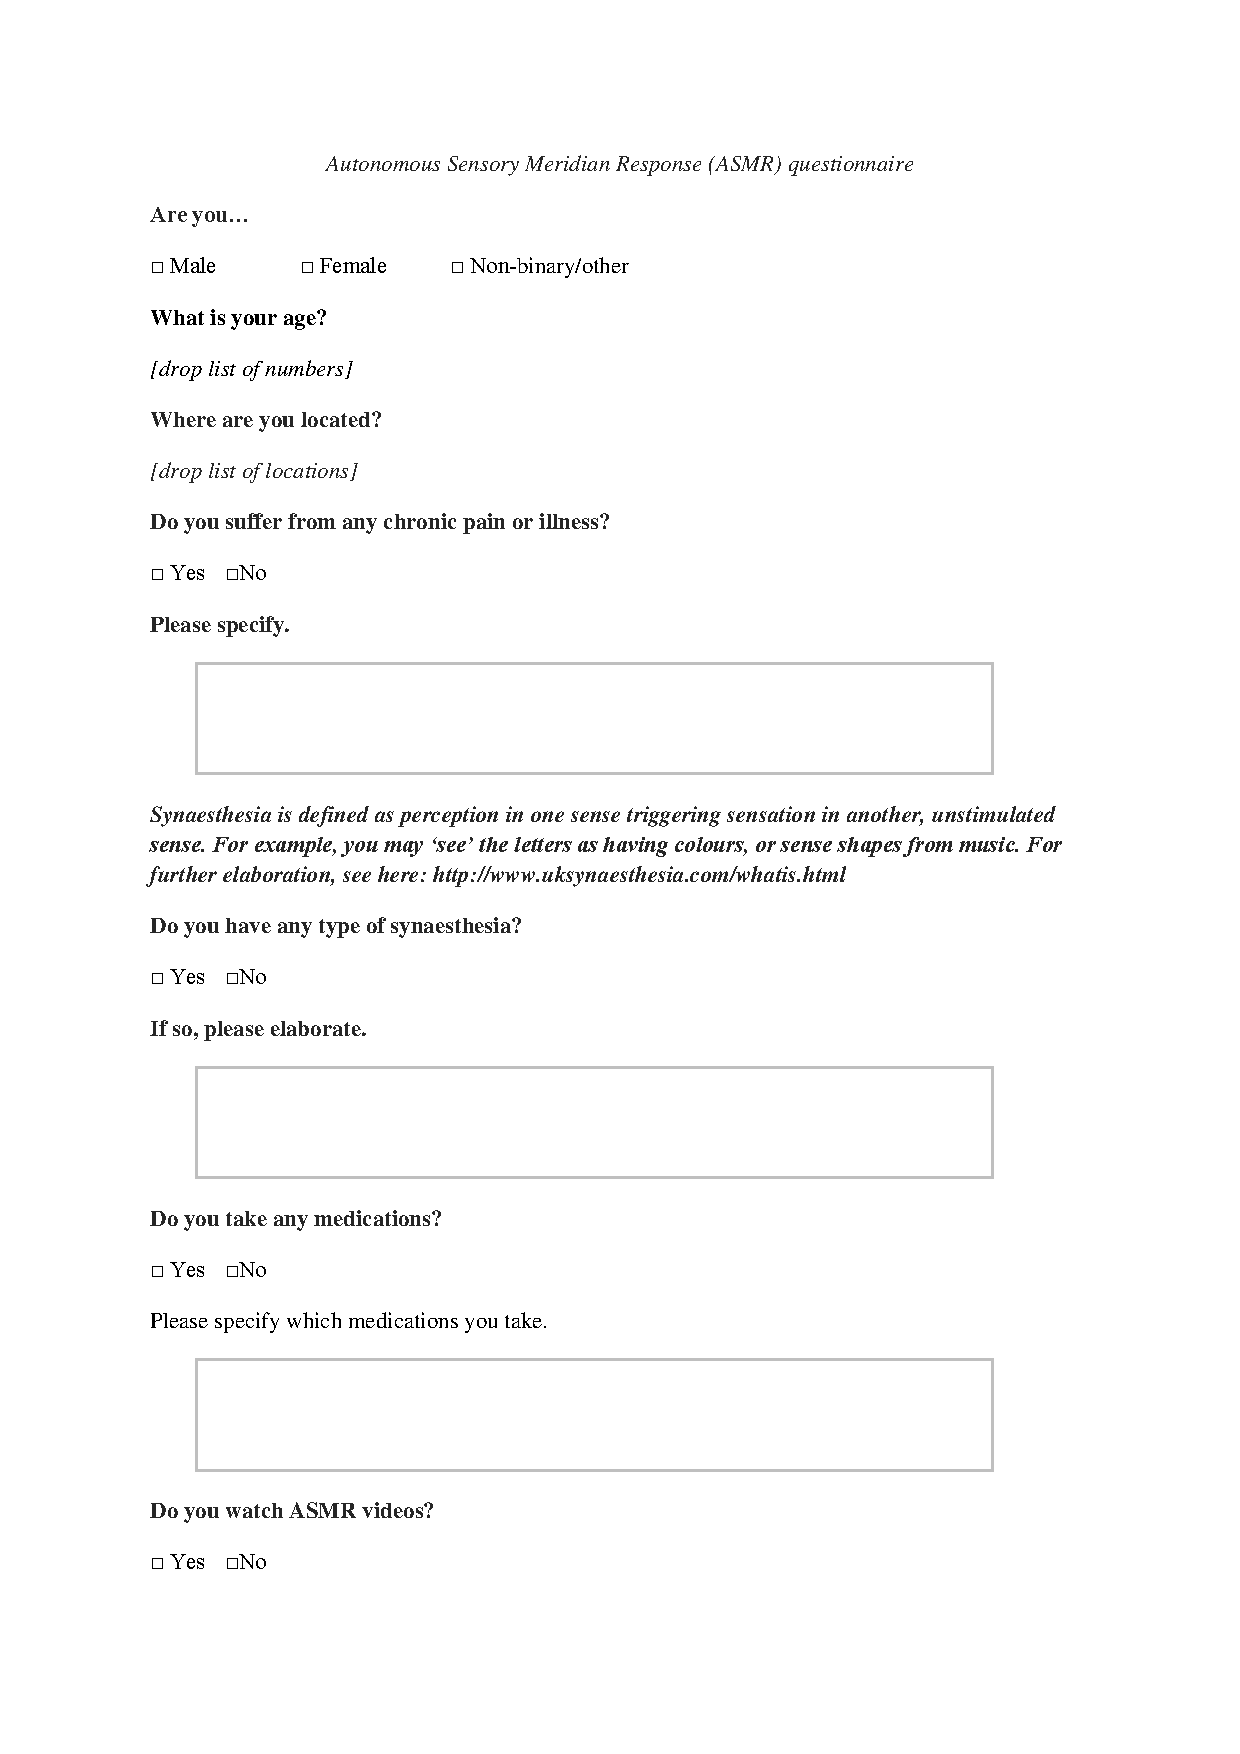
\includepdf[pages={1-}]{questionnaires/ASMR_Questions.pdf}


\end{document}

%%% Local Variables:
%%% mode: latex
%%% TeX-master: t
%%% End:
